
\chapter{Design and Implementation}
\label{cha:implementation}

intro...


\section{Decomposition Approach}

Decomposition describes the task of grouping nanoentities into services. Achieving a good solution according to the defined Coupling Criteria as described in \ref{sec:decompositionRequirements} requires a non trivial algorithm. This section documents the evaluation process for such an algorithm.

\subsection{Approach \#1: Clustering of a Weighted Undirected Graph}
\label{subsec:approach1_graph}

Our first approach to solve the decomposition problem was a clustering or community algorithm applied on a weighted, undirected graph.

Every nanoentity in the model is represented by a node. Edges define a relationship between two nanoentities. The weight on each edge shows how \textit{close} or \textit{cohesive} two nanoentities are. The higher the weight, the more likely they should belong to the same service. Figure \ref{fig:weighted_graph} shows an abstract example of such a graph.

\begin{minipage}[t]{0.5\textwidth}
\setlength{\parskip}{5pt plus 0.1pt}
	Figure \ref{fig:graph_approach} outlines a solution sketch for this approach. User representations such as class diagrams or use cases are imported. The \textit{importer} component extracts the nanoentities and the occurences of coupling, called Coupling Criteria Instances, in this model and stores this information into the database.
	
	The \textit{Solver} then creates all vertices from the nanoentities and builds edges between them according to the stored Coupling Criteria instances. This task is complex for the following reasons:
	
	\begin{enumerate}
		\item Coupling Criteria are not homogeneous as described in Section \ref{subsec:couplingCriteriaTypes}. 
		%TODO: write first about types before completing this item. Mention distance, closeness and cumulative criteria
		
		\item All Coupling Criteria information is reduced to a single number with one single unit of measurement. An increase of the weight for one Criteria automatically changes the relative importance of that CC to others.
		
		\item To allow the user to define the specific requirements of his system, priorities per Coupling Criteria can optionally be defined to influence the weights of each Coupling Criteria instance.
	\end{enumerate}
	
	The \textit{Clustering Algorithm} then analyzes the graph and creates clusters of nanoentities so that as few edges as possible need to be cut.
	
	\begin{figure}[H]
		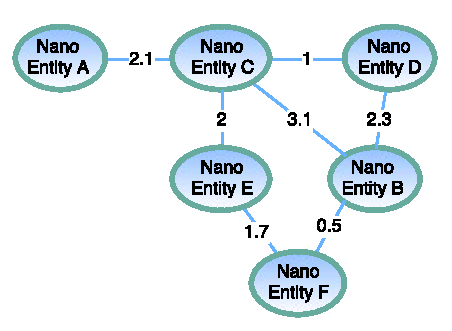
\includegraphics[scale=1.0]{diagrams/weighted_graph.pdf}
		\caption{Example of a Weighted Graph}
		\label{fig:weighted_graph}
	\end{figure}

\end{minipage}
\begin{minipage}[t]{0.5\textwidth}
	\begin{figure}[H]
		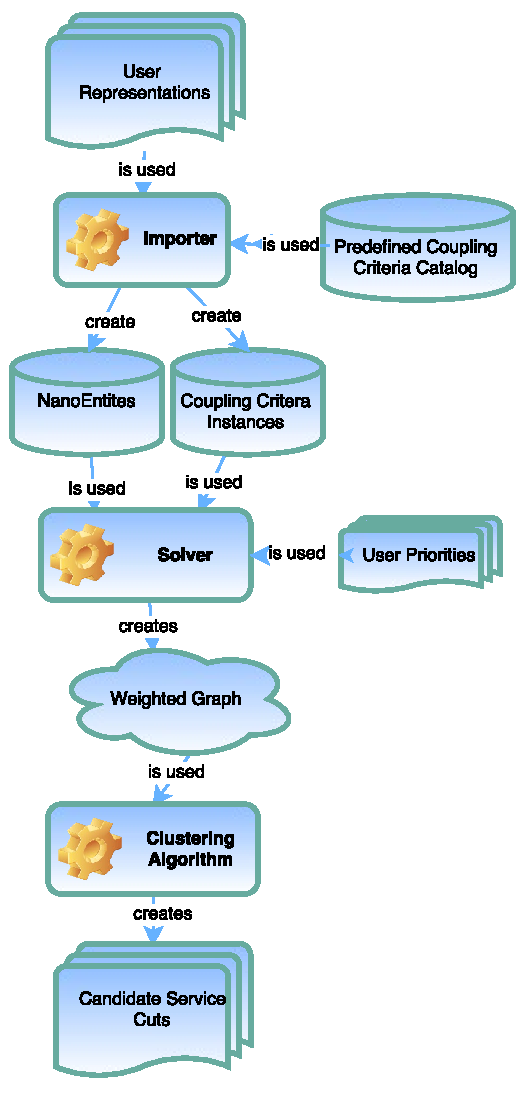
\includegraphics[scale=1.0]{diagrams/graph_approach.pdf}
		\caption{Solution Sketch for a Weighted Graph with a Clustering Algorithm}
		\label{fig:graph_approach}
	\end{figure}
\end{minipage}

A detailed evaluation of clustering algorithms is document in Appendix \ref{appendix:graphClustering}. We decided to do a first assessment of this approach using the \gls{MCL}\cite{markovCluster} and Girvan-Newman\cite{girvan} algorithms. Both algorithms are implemented as plugins of the Gephi\cite{gephi} platform and can be extracted as \gls{JAR} files.

\subsubsection{Practical Assessment of the Graph Clustering Approach}

To assess the graph approach we use a simple booking domain model. In Figure \ref{fig:clusteringBookingSimple} the MCL algorithm was tested using the booking model with all Coupling Criteria priorities set to zero except the \textit{Identity \& Lifecycle Commonality} Criteria. Consequently the visualized services contain one entity each. The entities can be identified as \textit{Customer}, \textit{Article} and \textit{Booking}.

\begin{figure}[H]
	\begin{center}
		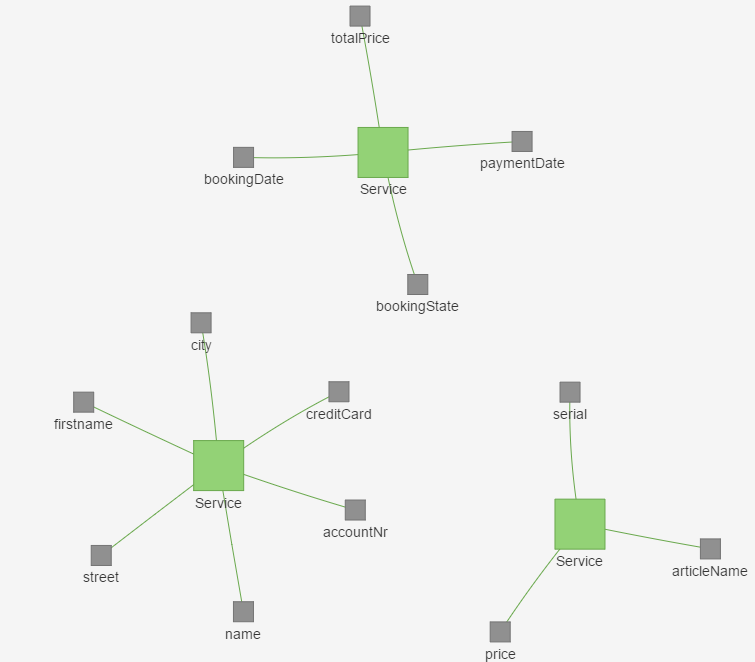
\includegraphics[scale=0.8]{images/booking_entities.png}
	\end{center}
	\caption{Clustering of a simple Booking example.}
	\label{fig:clusteringBookingSimple}
\end{figure}


Figure \ref{fig:clusteringBooking} demonstrates the result of the MCL algorithm with user stories of the Booking domain added. 

\begin{figure}[H]
	\begin{center}
		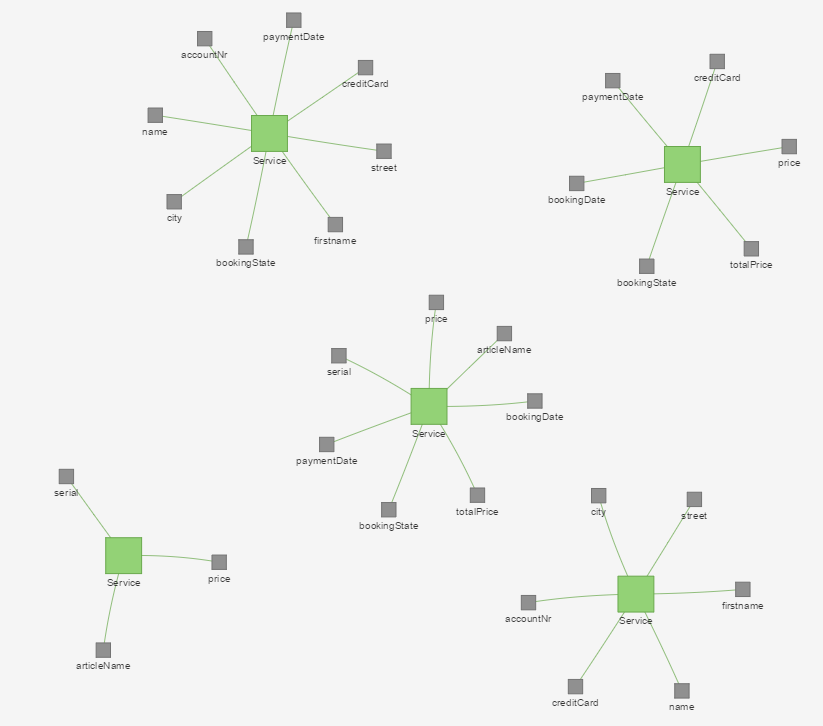
\includegraphics[scale=0.7]{images/booking_entities_mcl.png}
	\end{center}
	\caption{Booking Example enhanced with User Stories.}
	\label{fig:clusteringBooking}
\end{figure}

Obviously this is not the expected result. The service clusters are formed with nanoentities belonging to several clusters at the same time. Therefore the MCL algorithm cannot be used for our application.


\subsubsection{Discussion}

As proven with the first graph samples based on entity and use case relationships, the problem can be mapped to a graph. This allows to leverage existing graph clustering algorithms.

We identified two conceptional challenges of the graph approach. Firstly the theoretical number of nodes may cause performance problems and secondly a separation constraint can not directly modeled on a graph. The following paragraphs cover those problems.

A weighted graph can only describe how close two nanoentities are. This includes all coupling criteria of type cohesiveness. Coupling that describes separation or incompatibility, where different characteristics should be separated, can only be mapped to the graph indirectly as negative scores. %TODO müssen die positiven scores grösser sein als die penalties?

The maximum number of edged in a graph can be described using a formula: A graph of $n$ nodes, where every node is connected to all other nodes, has $e$ edges.

\begin{displaymath}
e = \frac{n(n-1)}{2}
\end{displaymath}

The number of edges grows almost quadratically as shown in Table \ref{tab:edgesCount}.

\begin{table}[H]
	\centering
	\caption{Maximum number of edges in an undirected graph}
	\label{tab:edgesCount}
	\begin{tabular}{|r|r|}
	\hline \textbf{Nodes} $n$ & \textbf{Edges} $e$ \\ 
	\hline 2 & 1 \\ 
	\hline 3 & 3 \\ 
	\hline 20 & 190 \\ 
	\hline 50 & 1'225 \\ 
	\hline 100 & 4'950 \\ 
	\hline 2000 & 1'999'999 \\ 
	\hline 
	\end{tabular} 
\end{table}

Our implementation however will unlikely have anything close to the theoretical number of edges as:
\begin{itemize}
\item Coupling of type \textit{Cohesiveness} only adds edges where nanoservices are in a relationship with each other.
\item Coupling of type \textit{Compatibility} only adds a negative score (penalty) to existing relationships.
\item Coupling of type \textit{Constraint} only removes existing edges.
%todo communication
\end{itemize}

The number of edges can therefore only cause problems when a Cohesiveness coupling is specified that includes a large number of nodes. An example of such a coupling is for a use case including a very large number of nanoentities which is a very unlikely case. We therefore conclude that the number of edges is probably not an issue.



\subsection{Approach \#2: Rating of possible Service Cuts}

During sprint 2 we conducted a feasibility assessment with a professor of mathematics of the graph based approach as documented in Appendix \ref{sec:feasibilityAssessment}. The result of the assessment is the idea to create a set of all possible service cuts and rate the cuts isolated per Coupling Criteria. The approach is illustrated in Figure \ref{fig:setProcess}.

\begin{figure}[H]
	\begin{center}
		\includegraphics[scale=0.45]{diagrams/scoring_process.png}
	\end{center}
	\caption{Approach \#2: Set Rating}
	\label{fig:setProcess}
\end{figure}

This approach is processed in three steps:

\begin{description}
	\item[Partitioning] Based on the nanoentities, a set of all possible candidate service cuts is calculated. This includes every theoretically possible service cut for every number of services. For practical usage, this step needs to be optimized. 
	\item[Assessment] For all Coupling Criteria a processor assesses all service cuts with a score describing how well the criteria's requirements are met. The score is a number between 0 and 10, while 10 means that all requirements are perfectly satisfied. 
	\item[Evaluation] The user optionally defines priorities how important each Criteria is for his system. The priorities are defined with approximately exponential numbers like the Fibonacci sequence. These priorities are applied on the service cut scores. The resulting best candidate cut is then presented to the user.
\end{description}

\subsubsection{Discussion}

An advantage of this approach is that each relevant step is clearly separated and can thus be analyzed, debugged and visualized better than in the graph based approach. The assessment and score calculation is done separately for every cut and for every Coupling Criteria. Each Criteria processor needs to score candidate cuts with a uniform scoring range. 

The weak point is the partitioning process. Theoretically every possible set of services where each nanoentity is contained in one and only one Service is a candidate cut. In mathematics this is described as the \textit{partition of a set}\cite{partitionOfASet} problem. The Bell number $B_n$ defines the amount of possible partitions: 


\begin{displaymath}
B_{n+1}=\sum_{j=0}^n {n\choose j} B_j
\end{displaymath}

For the Service Cutter $n$ is the number of nanoentities, so the number of possible service cuts for $n=20$ nanoentities is $51'724'158'235'372$\footnote{We don't show the number for the required $2000$ nanoentities for lack of space in the document.}.

The Bell number includes cuts for $1 - n$ number of Services. In the context of a software system only certain numbers of Services are realistic. The \textit{Stirling numbers of the second kind} calculate the Bell number for a given number of sets $k$:

\begin{displaymath}
\left\{ {n \atop k}\right\} = \frac{1}{k!}\sum_{j=0}^{k} (-1)^{k-j} \binom{k}{j} j^n
\end{displaymath}

For $n=20$ nanoentities and $k=4$ Services the equation results in $45'232'115'901$ possible cuts. For $k=6$ its already $4'306'078'895'384$.

During a discussion with our industry partner and supervisor documented in Appendix \ref{sec:status22102015}, we decided that the Service Cutter should be able to process system models with up to 2000 nanoentities. We therefore concluded in the same meeting that this approach is not practicable without a heuristic approach of finding a small set of relevant candidate cuts. 

A possible heuristic approach is to take one or a few Coupling Criteria information about the system into account for finding Service Candidates. A simple example would be to only analyze cuts where nanoentities of the same entity are not split across services so that only entities and not it's nanoentities need to be considered.

As we tried to find a heuristic approach to calculate candidate cuts, we discovered a new idea for the composition algorithm described in the next approach. 

\subsection{Approach \#3: Constructing Services - a Heuristic Approach}

(Notes only)
Idee:

Distanzkriterien: Umso mehr Services umso besser die Lösung (Nanoservices)
Nähekriterien: Umso weniger Services umso besser die Lösung (Monolith)

Die richtige Anzahl Services ist eine kritische Dimension der Lösung, welche unter anderem aber von vielen externen (z.B Infrastruktur) Faktoren abhängt. Entscheidung: Die Verantwortung für das bestimmen der Anzahl Services an den User auslagern.

Nun ist es möglich eine bestimmte Anzahl Services zu füllen. Dazu kann ein heuristischer, empirischer Algorithmus mit intelligentem Rütteln genommen werden. 
Jede Verbindung von zwei Feldern wird von jedem CC mit einer einheitlichen Einheit bewertet. Dadurch kann einfach bestummen werden, wie gut ein Feld in ein Topf passt. Alle Töpfe werden gefüllt (wenn es nirgends passt in den kleinsten Topf). Danach wird angefangen Feldern die am wenigsten passen in einen anderen Topf zu werfen.
Der Algorithmus kann beliebig(?) weiterlaufen und optimieren. Wenn der Algorithmus gut funktioniert, kann man während der Optimierung auch die Gewichtung anpassen und schauen was damit passiert.
Idee: Snapshots machen von Status bevor eine Gewichtung angepasst wird.
Idee: Am Anfang 5 Minuten durchlaufen, 10 Vorschläge ausarbeiten und dann den user entscheiden lassen auf welchen er weiter optimieren will (?) Evtl. kann auch der Algorithmus entscheiden indem er die lösungen vergleicht? 

Weitere Idee: Aufsplitten auf logische (A) und physische (B) Kriterien und Decomposition mode? Kann der Algorithmus in zwei Schritten geschehen? Bzw. lösen wir eigentlich 2 Probleme (Logisch \& Physisch) auf einmal?


\section{Clustering Algorithm}

We decided to use the clustering algorithms Girvan-Newman and Leung. Both provide the required functionality and should support on clusters with up to 2000 nodes. %TODO is leung a bit faster? test!

The \gls{MCL} algorithm according to the paper\cite{markovCluster} supports the desired functionality. However we did not find a stable Java implementation of it and therefore did not test it in detail.

A full comparison of the evaluated algorithms is attached in Appendix \ref{appendix:graphClusteringAlgs}.

\subsection{Girvan-Newman}

M. E. J. Newman and M. Girvan\cite{girvan} proposed to use a divise approach to graph clustering. This approach repeatedly finds the least connected pair of nodes and removes the edges between them. This process divides the graph into smaller and smaller components and can be stopped at any time to select the components at this time to be the graph clusters.

In the ordered graph in Figure \ref{fig:girvan-newman-process} Girvan-Newman would remove the edges in ascending order. The graph is split into 4 clusters after 4 iterations.

Girvan-Newman stops as soon as the desired number of clusters has been reached.

\begin{figure}[H]
	\begin{center}
		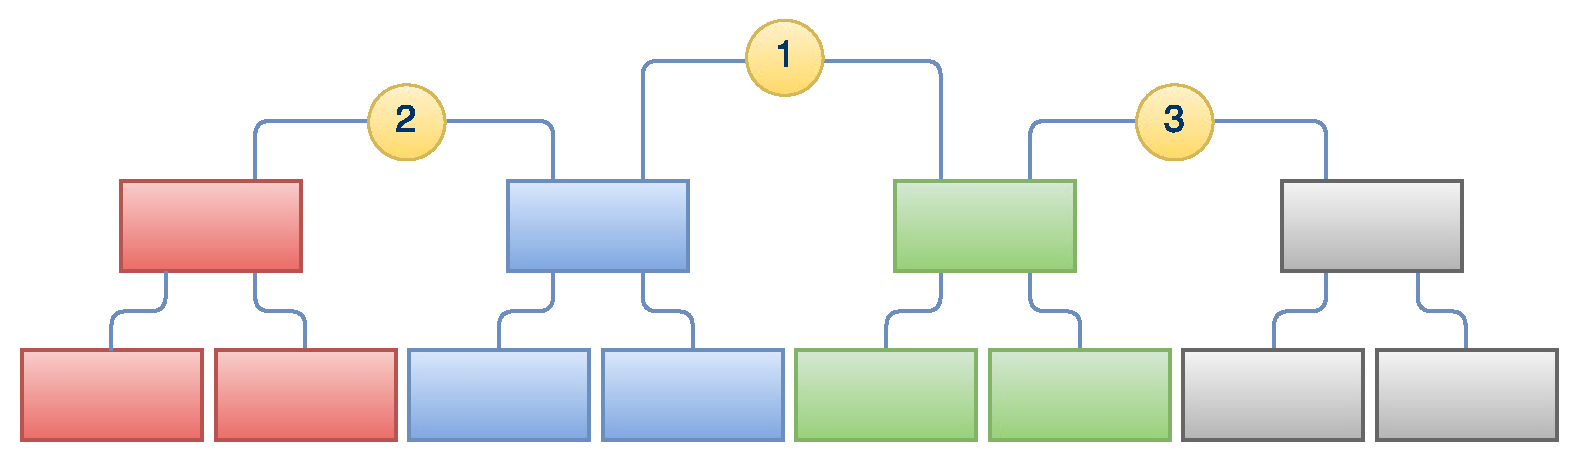
\includegraphics[scale=0.45]{diagrams/Girvan-Newman-Process.pdf}
	\end{center}
	\caption{Girvan-Newman forms clusters by removing edges iteratively}
	\label{fig:girvan-newman-process}
\end{figure}

As this algorithm does not include random elements, the proposed clusters are always identical.

\subsection{Leung}

In 2009 Leung \textit{et al}\cite{leung} refined the \enquote{Epidemic Label Propagation} algorithm as proposed by Raghavan \textit{et al}\cite{raghavan} in 2007. 

Raghvan described the algorithm as follows: \enquote{Each node in the network chooses to
join the community to which the maximum number of its neighbors belong to, with ties broken uniformly randomly. We initialize every node with unique labels and let the labels propagate through the network. As the labels propagate, densely connected groups of nodes quickly reach a consensus on a unique label.}\cite[p. 4]{raghavan}.

Leung further refined the algorithm by adding a \enquote{Hop Attenuation Factor} $\delta$ to prevent labels from spreading across two clusters. He explains: \enquote{The value $\delta$ governs how far a particular label can spread as a function of the geodesic distance from its origin. This additional parameter adds in extra uncertainties
to the algorithm but may encourage a stronger local community to form before a large cluster start to dominate.}

Leung does not specify an order in which nodes are to be processed. Therefore the labels may spread differently in repeated runs. We witnessed varying clusters while testing the Service Cutter. %TODO add reference to ddd sample chapter

\section{Scoring}

The scoring process rates the relation of two nanoentities with a score. A higher positive score states that these entities should be modeled in the same service while a negative score asks for a separation of the nanoentities into different services.

\begin{figure}[H]
	\begin{center}
		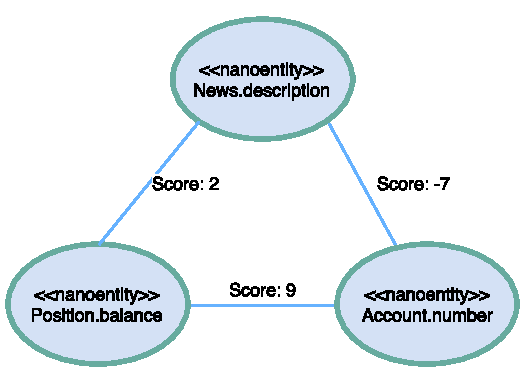
\includegraphics[scale=1]{diagrams/scoring_example.pdf}
		\caption{Simple Scoring Example}
		\label{fig:scoringExample}
	\end{center}
\end{figure}

Figure \ref{fig:scoringExample} shows three nanoentities from the Trading System (see Appendix \ref{sec:tradingSystem}) and their scores to each other. The relation \textit{Position.balance} to \textit{Account.number} has a high score as these nanoentities are often accessed in the same use cases and therefore get a high score from the \textit{Semantic Proximity} criterion. \textit{News.description} to \textit{Account.number} has a negative score. These nanoentities do not have common use cases and do not belong to the same entity, so the positive scores from \textit{cohesiveness} criteria are low or zero. Different characteristics like \textit{low} resilience requirements for \textit{News.description} and \textit{critical} resilience requirements for \textit{Account.number} lead to a negative score. 

In this simple example, the Service Cutter would most probably suggest two services, one with \textit{Account.number} and \textit{Position.balance} and another one with the \textit{News.description}.

To determine the final score between two nanoentities three steps are required. First every coupling criterion scores the relations it has information about. After that, priorities for each criterion are applied. Finally the prioritized scores of all criteria are summed up to a final score.

\subsection{Step 1: Score by Coupling Criterion}

Every coupling criterion calculates a score between $-10$ and $10$ for each nanoentity relation $AB$. 

\begin{displaymath}
criteria[i].score_{AB} = -10 ... 10
\end{displaymath}

A score of $10$ implies that \enquote{From the view of coupling criterion $i$, the nanoentities $A$ and $B$ should definitly reside in the same service.} A score of $-10$ implies that \enquote{From the view of coupling criterion $i$, the nanoentities $A$ and $B$ should definitly \textbf{not} reside in the same service.} 

The range from $-10$ to  $10$ was chosen to be able to compare scores of different coupling criterion with each other. A fixed range guarantees that not one criterion receives more importance than another one due to its scoring logic. Other ranges like $-1.00$ to $1.00$ would have worked as well, but in our opinion integer numbers are easier to understand for users than rational numbers. 

It is important to notice that not every criterion has to use the full possible range. Coupling criteria of type \textit{cohesiveness} tend to score only positive values, as they describe why nanoentities should be composed in the same service. Criteria of type \textit{compatibility} or \textit{constraints} on the other hand tend to score negative, as they describe reasons to split nanoentities into different services.

\subsection{Step 2: Prioritized Coupling Criteria}

In the second step, the coupling criteria are prioritized relatively to each other. Table \ref{tab:priorities} outlines all possible priorities.

\begin{table}[H]
	\centering
	\caption{Coupling Criterion Priorities}
	\label{tab:priorities}
	\begin{tabular}{|p{70pt}|p{30pt}|}
		\hline	
		Representation & Value  \\
		\hline
		IGNORE & 0  \\
		\hline
		XS & 0.5  \\
		\hline
		S & 1  \\
		\hline
		M & 3  \\
		\hline
		L & 5  \\
		\hline
		XL & 8  \\
		\hline
		XXL & 13  \\
		\hline
	\end{tabular}
\end{table}

The priorities are represented by t-shirt sizes each defining a priority value. By recommendation of Zühlke and inspired by agile estimation scales\footnote{Alex Yakyma wrote an interesting paper on why progressive estimations are efficient for teams\cite{estimation}.}, we chose a progressive and nearly exponential value sequence. 

Having very high values allows analyzing a system in the Service Cutter with focus on one or two coupling criteria only as giving a criterion the priority XXL quickly makes it more important than many of the other criteria together. With progressive values we obtain this ability while still keeping the number of priorities small in order to make it simpler to map each criterion to a priority. 

The priority of each criterion is multiplied with all scores given by that criterion. 
\begin{displaymath}
	criteria[i].prioritizedScore_{AB} = criteria[i].score_{AB} * criteria[i].priorityValue
\end{displaymath}

It is important to distinct between a criterion score (step 1) and a prioritized score (step 2). A criterion score is a statement on the relation of two nanoentities per coupling criterion where each coupling criterion has the same importance ($-10$ to $10$). The prioritized score multiplies this statement by the importance of the criterion in the analyzed system. Priorities are very context sensitive. Priorities of a real-time entertainment system will have for example very different priorities than a system handling financial transactions. 

\subsection{Step 3: Final Relation Score}

The final relation score between two nanoentities is the sum of all prioritized scores per coupling criterion: 

\begin{displaymath}
finalScore_{AB} = \sum\limits_{i=1}^n criteria[i].score_{AB} * criteria[i].priorityValue_{AB}
\end{displaymath}

The undirected weighted graph is then built with each vertex representing a nanoentity. Nanoentity relations with a positive score are connected by an weighted edge:

\begin{displaymath}
edgeWeight_{AB} = max(0, finalScore_{AB})	
\end{displaymath}

Negative scores are not represented on the graph. Negative scores request a separation of nanoentities in different services. This information is lost in the graph based approach. Nevertheless, we have not encountered actual problems from this as clustering algorithms are unlikely to put two vertices in one cluster that do not have a connecting edge.
	
\subsection{Default Priorities}
\label{sec:defaultPriorities}

\begin{minipage}[t]{0.5\textwidth}
\setlength{\parskip}{5pt plus 0.1pt}

%TODO: sinnvollere defaults definieren? XS for security constraint ist wohl nicht so gut. 
One problem the scoring system has is that the sum in step 3 adds together positive and negative scores. If the amount of criterion give negative scores is high, the likelihood to reach a negative final score gets bigger. While analyzing test systems documented in Appendix \ref{testSystems}, we found default priorities as shown in Figure \ref{fig:priorities} provide reasonable results.


Default priorities: \newline
Cohesiveness criteria: M\newline
Compatibility criteria: XS\newline 
Constraints criteria: M\newline

\end{minipage}
\begin{minipage}[t]{0.6\textwidth}
	\begin{figure}[H]
		\begin{center}
			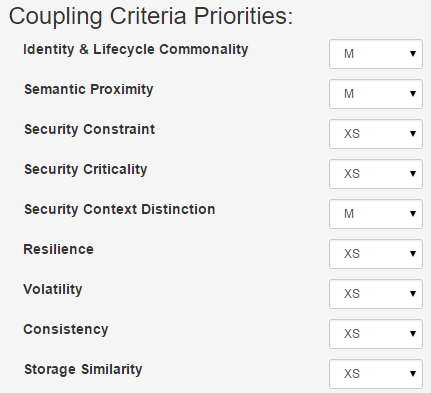
\includegraphics[scale=0.5]{images/priorities.png}
			\caption{Screenshot of Default Priorities in the Service Cutter}
			\label{fig:priorities}
		\end{center}
	\end{figure}
\end{minipage}

\subsection{Scoring Logic}

This section documents how each coupling criterion calculates its criterion score from $-10$ to $10$. 

Figure \ref{fig:scorer} shows the CriterionScorer interface used to calculate criterion scores. 

%TODO update
\begin{figure}[H]
	\begin{center}
		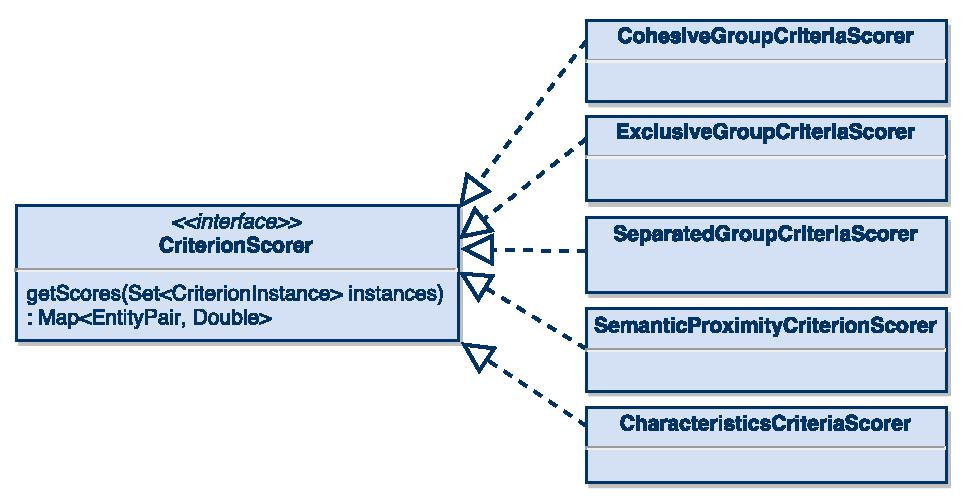
\includegraphics[scale=0.7]{diagrams/scorer.pdf}
		\caption{CriterionScorer Interface and its implementations}
		\label{fig:scorer}
	\end{center}
\end{figure}

Currently there are four CriterionScorer implementations for different coupling criteria. Not all criteria have a suitable implementation yet, as we prioritized the criteria during the project as there was not enough time to implement the scoring for all criteria. Table \ref{tab:scorer} outlines which implementation is used for which coupling criterion.

\begin{table}[H]
	\centering
	\caption{Coupling Criteria and their Scorer Implementation}
	\label{tab:scorer}
	\begin{tabular}{|p{170pt}|p{200pt}|}
		\hline	
		\textbf{Coupling Criteria} & \textbf{Scorer Implementation}  \\
		\hline
		Responsibility \newline Consistency Constraint \newline Identity \& Lifecycle Commonality  & CohesiveGroupCriteriaScorer \\
		\hline
		Predefined Service Constraint  & ExclusiveGroupCriteriaScorer \\ 
		\hline
		Security Constraint & SeparationCriteriaScorer \\
		\hline
		Semantic Proximity & SemanticProximityCriterionScorer \\
		\hline
		Change Similarty \newline Consistency \newline Resilience \newline Volatility \newline Storage Similarty \newline Security Criticality & CharacteristicsCriteriaScorer  \\
		\hline
		Mutability \newline Network Traffic Suitability \newline Latency \newline Security Contextuality & No Implementation  \\
		\hline
	\end{tabular}
\end{table}

\subsubsection{CohesiveGroupCriteriaScorer}

A CohesiveGroupCriteriaScorer is used for the criteria \textit{Consistency Constraint}, \textit{Identity \& Lifecycle Commonality} and \textit{Responsibiltiy}. These criteria define one or more groups of nanoentities that for some reason should be kept together in one service.

The scorer sets the maximum score of $10$ for every relation between nanoentities inside a group. 

\subsubsection{ExclusiveGroupCriteriaScorer}

A ExclusiveGroupCriteriaScorer is used for the \textit{Predefined Service Constraint} criterion. The scorer implements the same logic as a CohesiveGroupCriteriaScorer, but additionally sets a penalty of $-10$ from a nanoentity inside a group to all other nanoentities which do not share the same group.

\subsubsection{SeparationCriteriaScorer}

A SeparationCriteriaScorer is used for the criterion \textit{Security Constraint}. The criterion defines two or more groups of nanoentities which should clearly be separated into different services for security reasons. 

The implementation sets a negative score of $-10$ from each nanoentity to all other nanoentities defined in other groups than the own one. 

\subsubsection{SemanticProximityCriterionScorer}

%TODO: name for UML diagram? 
The SemanticProximityCriterionScorer is a more complex scoring implementation. It considers use cases and aggregations within a UML diagram. To calculate the score, the scorer uses an intermediate score summing up occurrences of the following conditions for the nanoentities $A$ and $B$:

\begin{description}
	\item [READ\_ACCESS] $A$ and $B$ are both read in the same use case.
	\item [WRITE\_ACCESS] $A$ and $B$ are both written in the same use case.
	\item [MIXED\_ACCESS] One of $A$ or $B$ is read and the other one written in the same use case.
	\item [AGGREGATED\_ENTITY] $A$ belongs to an entity which has an aggregation to B's entity in UML diagram. 
\end{description}

For each occurrence a number is added to the intermediate score of the $AB$ relation. Currently the following numbers are implemented:

SCORE\_WRITE\_ACCESS: 10 \newline
SCORE\_READ\_ACCESS: 3  \newline
SCORE\_MIXED\_ACCESS: 3 \newline 
SCORE\_AGGREGATION: 1 \newline 

These values are only used for the intermediate score and are not to be confound with the criterion score of $-10$ to $10$. More important than the actual numbers are the relative differences to each other which define the importance of the occurrences. Our defaults listed above put a strong emphasis on mutual write access. 

To reduce the intermediate score to the criterion score, the following rules are applied:

\begin{itemize}
	\item The top 10\% of all relations with the highest intermediate score receive a criterion score of 10.
	\item The lowest intermediate score of the top 10\% defines the reference intermediate score. The other 90\% are calculated relatively to that reference and receive a criterion score between 0 and 10.
\end{itemize}

The calculation for the lower 90\% works as following:

%TODO Michi: verstehe ich nicht!

\begin{equation}
\frac{referenceIntermediateScore}{x} = 10
\end{equation}
\begin{equation}
x = \frac{referenceIntermediateScore}{10}
\end{equation}
\begin{equation}
criterionScore_{AB} = \frac{intermediateScore_{AB}}{X}
\end{equation}

Both, the numbers counted for access or aggregation occurrences and the reduction to the criterion score have been experimental evaluated. The algorithm documented here has proven to produce reasonable results for the example systems tested but might require further investigations for other systems. 

\subsubsection{CharacteristicsCriteriaScorer}
%TODO styles?

Each coupling criterion of type compatibility defines multiple characteristics. The idea of these criteria is to create services with as homogeneous nanoentities as possible. The scorer therefore sets negative scores for a relation between two nanoentities having different characteristics. 

As an example, the criterion \textit{Change Similarity} describes how often change requests need to be implemented that affect a nanoentity. A nanoentity can have the characteristic \textit{often, normal} or \textit{rarely}. Each characteristic has a number between $0$ and $10$ assigned:

Often: $10$ \newline
Normal: $4$ \textit{(default)} \newline
Rarely: $0$ \newline

Two nanoentities with different characteristics receive a negative score with the difference between the numbers. As an example, a nanoentity $A$ with characteristic \textit{often} and a nanoentity $B$ with characteristic \textit{normal} receive a criterion score of $-6$. 

It is important that the highest and lowest number have a difference of $10$ to fully use the range a criterion has to rate a relation. \newline In this case there is an intermediate value of $4$ for the \textit{normal} characteristic. In our experience the often changing nanoentities are the most interesting and have the highest impact on service decomposition. With using the number $4$ instead of $5$ for \textit{normal} we put an emphasis on \textit{often} as the differences to this characteristics become bigger. 

To improve usability we introduced default values so that a user does not need to define characteristics of all criteria for all nanoentities. 

Table \ref{tab:characteristics} outlines characteristics of all criteria with their values and defaults. Both, the numbers and defaults are configurable for advanced users to better suit a systems requirements. 

\begin{table}[H]
	\centering
	\caption{Criteria Characteristics with values and defaults}
	\label{tab:characteristics}
	\begin{tabular}{|p{100pt}|p{80pt}|p{60pt}|}
		\hline	
		\textbf Criterion & Characteristics & Default\\
		\hline
		Change Similarity & Often 10 \newline Normal 4 \newline Rarely 0 & Normal\\
		\hline
		Consistency & High 10 \newline Eventually 3 \newline Weak 0 & High\\
		\hline
		Resilience & Critical 10 \newline Normal 4 \newline Low 0 & Normal\\
		\hline
		Volatility & Often 10 \newline Regularly 5 \newline Rarely 0 & Regularly \\
		\hline
		Storage Similarity & Huge 10 \newline Normal 3 \newline Tiny 0 & Normal\\
		\hline
		Security Criticality & Critical 10 \newline Internal 3 \newline Public 0 & Internal\\
		\hline
	\end{tabular}
\end{table}


\section{Prototype} 

This section introduces the prototypical implementation of the Service Cutter to verify the feasibility of the decomposition approach presented in the previous section.

\subsection{Design}

The design of the Service Cutter was intentionally not evaluated in detail. We therefore followed the recommendation of our industry partner and used Spring Boot\cite{springboot} and JHipster\cite{jhipster} as the underlying frameworks.

The main reasons were:

\begin{itemize}
\item Zühlke uses them successfully.
\item Spring Boot is considered the way to go for Spring based applications nowadays.
\item JHipster is based on established technologies that are partially already familiar to us. Furthermore it provides a code generator and samples. This can noticeable speed up development especially in the prototyping area.
\item We were able to implement a technological proof of concept in a few days and did not face major obstacles.
\end{itemize}

For the reasons listed above, we implemented the web application component using JHipster and the Engine using Spring Boot combined with a web service library. Section \ref{subsec:technology} discusses the utilized technologies in more detail.

\subsection{Technology}
\label{subsec:technology}


\begin{minipage}[t]{0.5\textwidth}
\setlength{\parskip}{5pt plus 0.1pt}
	The Service Cutter is implemented as a three tier application.
	
	The first tier is the web \textit{browser} of the user. The single-page application is based on AngularJS\cite{angularjs} and uses a template based on Bootstrap\cite{bootstrap}. A REST API provides access to the Editor tier.
	
	The \textit{Editor} component is a web application based on the JHipster\cite{jhipster} framework. It provides the use the possibility to import this domain information using a JSON upload and feeds this information into the Engine. All security and user interface aspects are handled in this layer.
	
	The Engine is the isolated component that holds all the code to calculate service decomposition suggestions. It is also based on Spring technologies and provides a REST web service. The Engine does not provide any security measures and it is therefore necessary to restrict access to the Engine. We recommend to achieve this using a Docker\cite{docker} internal network as described in Section \ref{subsec:infrastructure}.
	
	%TODO db/orm? -> spring data supports hibernate
	
\end{minipage}
\begin{minipage}[t]{0.5\textwidth}
	\begin{figure}[H]
		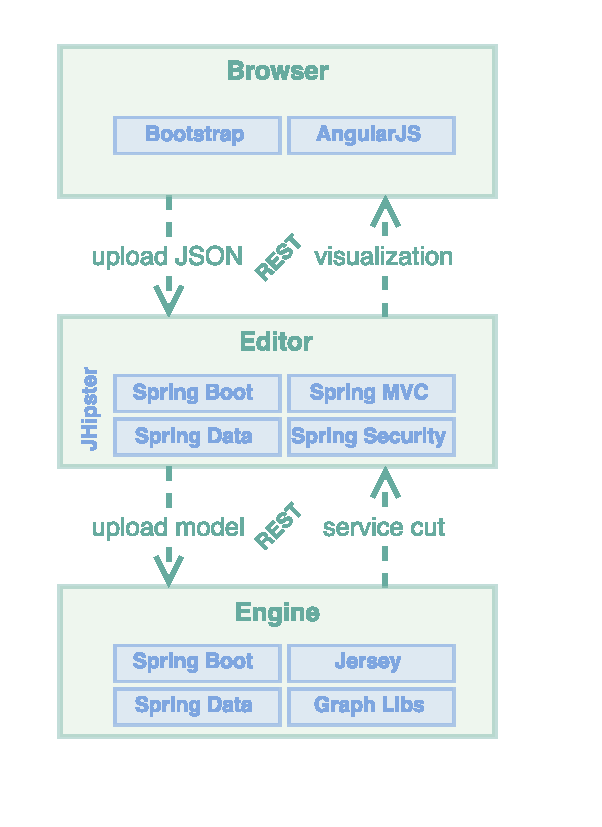
\includegraphics[scale=1]{diagrams/Technologies.pdf}
		\caption{Technology overview}
		\label{fig:technologies}
	\end{figure}
\end{minipage}


\subsection{Infrastructure}
\label{subsec:infrastructure}

Technically the Service Cutter can be operated on a single server providing a relational database and a Tomcat web server. However we developed a more sophisticated infrastructure aligned with modern standards which is presented as follows.

\begin{itemize}
\item Every components runs in an isolated Docker\cite{docker} container.
\item Docker Compose\cite{dockercompose} is used to link the Docker containers (hostnames, ports).
\item The Engine and the Editor operate in an embedded Tomcat server as provided by Sprint Boot web.
\item The Engine and the Editor both require a relational database. As Hibernate\cite{hibernate} and Liquibase\cite{liquibase} are used, all database related code is vendor agnostic. However we only tested the Service Cutter on Postgres 9.4\cite{postgres}.
\end{itemize}

The Docker Compose definition is attached in Appendix \ref{appendix:dockerCompose}.


\subsection{Graph Analyzing}

\begin{figure}[H]
	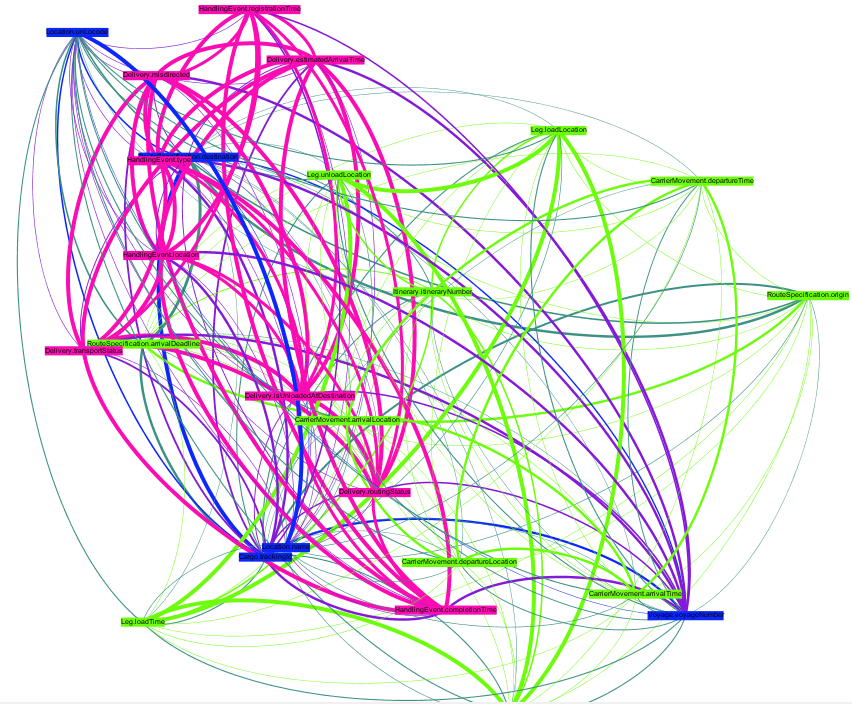
\includegraphics[scale=0.7]{images/ddd_semantic_proximity_debug.png}
	\caption{DDD Sample Graph Visualization with Gephi Platform}
	\label{fig:dddSampleGraph}
\end{figure}

\begin{figure}[H]
	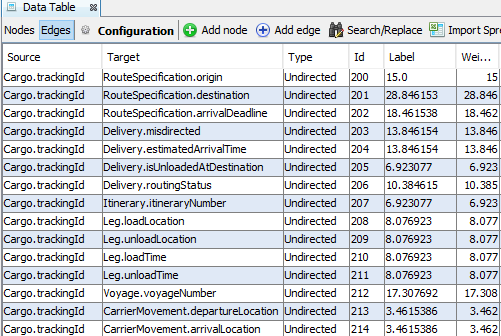
\includegraphics[scale=0.8]{images/ddd_semantic_proximity_debug_data.png}
	\caption{DDD Sample Graph Data Visualization with Gephi Platform}
	\label{fig:dddSampleData}
\end{figure}


\subsection{Information Security}

The web application is secured using an authentication and authorization implementation. Any other internal components such as the database or web services are hidden behind the servers firewall and therefore do not need any special security measures.

The uploaded data models are initially shared amongst all registered users.

\subsection{User Interface}

The base layout is responsive and adapts to smaller screens such as smartphones. However the tool is mostly used on devices such as laptops and the controls are therefore optimized for use on screens that are at least 15 inches wide and used with a mouse and a keyboard.


\bigskip
After covering the important design and implementation aspects, the next chapter assesses the built solution described in this chapter against the defined requirements.
